\chapter{Optional Libraries to be Linked into FHI-aims}
\label{appendix_external_packages_and_variants}

A core principle for FHI-aims is that it should be possible to build
all essential functionality with only a minimal set of dependencies,
typically a Fortran compiler, BLAS and LAPACK libraries, an MPI
library, and the ScaLAPACK library. These packages are essential for
performance and usually available on every relevant supercomputer
architecture. 

We note that while it is often easy to fulfil other,
far more complex dependencies on standard Linux type systems with
household tools, this is not always true for highly specialized
supercomputers. Yet, that computer may be precisely one the
multi-million dollar machine which would help solve an advanced
scientific problem. It is essential that a mere human be able to
compile FHI-aims with the appropriate performance on such a machine. 

That said, it may be beneficial to connect other libraries to FHI-aims
for special purposes, including libraries which require
cross-compilation with a C compiler. This section is intended to be
developed into a list of such libraries. Please also see Section
\ref{cross-compile-c} for some basic information.

\section{Adding Optional Libraries into FHI-aims: Stubs}

The optional presence or absence of certain libraries from FHI-aims at
compile time means that the main FHI-aims code must be able to deal
with the possible absence of certain subroutine or function calls to
those libraries at compile time.

In many codes, this is handled by adding preprocessor statement. In
FHI-aims, preprocessor flags are \textbf{NOT} the way forward. The
simple reason is that a single preprocessor flag may remain
understandable for an ordinary user; the proliferation of ten or more
preprocessor flags will create a serious obstacle for others to obtain
a reasonably compiled code. Code that introduces preprocessor
statements into FHI-aims will be removed from the code base.  

In FHI-aims, the recommended way to optionally add or circumvent a
given library is by creating a ``stub'' file for those library calls
-- essentially, empty subroutines that inform a user that they should
not have ended up here with a given version of the code (i.e., without
linking to a certain external library). At compile time, an
appropriate flag in the Makefile and Makefile.backend should be
created that switches between the real external library (if available)
or the ``stub'' file. Please follow the example of ``Spglib'' below in
the Makefile and in Makefile.backend for more information. The
principle is simple and easy to apply for any other optional library.

\section{Spglib}
\label{app:spglib}
Spglib is a library for finding and handling crystal
symmetries, written by Atsushi Togo
(\textbf{http://spglib.sourceforge.net}). FHI-aims can be interfaced
to the spglib.  

So far, FHI-aims supports the determination
of the crystal symmetry for a given 
(periodic) geometry file and k-point reduction based on this analysis 
(local and semi-local functionals only). Theoretical background and 
keywords are described in Section \ref{sec:symmetry}.

Prerequisites: \\

spglib is written in C and therefore needs a C compiler with
appropriate options in addition to the usual Fortran compiler with
which FHI-aims is built. Please enable a C compiler and add the
appropriate compiler flags to the \texttt{Makefile} or
\texttt{make.sys} file as described in Section \ref{cross-compile-c}. 

Specifically for spglib, include in \texttt{Makefile} or \texttt{make.sys}:\\
  
\begin{verbatim}
    USE_SPGLIB = yes
\end{verbatim}

Ideally the spglib source files should be placed in the folder \texttt{external/spglib} 
contained within the \texttt{FHI-aims} source (src) directory.

\keydefinition{use\_symmetry\_analysis}{control.in}
{
  \noindent
  Usage: \keyword{use\_symmetry\_analysis} \option{.true. / .false.} \\[1.0ex]  
  Purpose: This flag activates the interface to the spglib to obtain 
  symmetry information for the provided geometry file once.
  The symmetry information is directly written after the geometry printout
  in the FHI-aims standard output. spglib needs to be compiled with FHI-aims 
  to get the output. \\[1.0ex]
  Default: \option{.true.} \\
}
\keydefinition{sym\_precision}{control.in}
{
  \noindent
  Usage: \keyword{sym\_precision} \texttt{value} \\[1.0ex]  
  Purpose: This value determines the accuracy for identifying symmetric atoms. 
  The lower the value, the more strictly the atomic positions must overlap.\\[1.0ex] 
  Default: $10^{-5}$
}

\section{Libxc}
\label{app:spglib}
Libxc is, accordingly to its website, ``a library of exchange-correlation functionals 
for density-functional theory. The aim is to provide a portable, well tested and reliable 
set of exchange and correlation functionals that can be used by all the ETSF codes and 
also other codes.''  More information may be found at \url{http://octopus-code.org/wiki/Libxc}.
The version distributed with the FHI-aims source code is 4.0.2.

At the time of this writing (28 January 2017), FHI-aims uses its own set of 
exchange-correlation functional implementations for the calculation of the 
exchange-correlation energy during the SCF cycle.  Compiling FHI-aims with 
Libxc support does not change this.  We provide users the option to compile 
with Libxc support because multiple developers have made use of Libxc in
their own code for extended functionality in FHI-aims, such as calculations of
NMR parameters and the atom\_sphere radial solver.  If a particular method 
requested by the user requires Libxc, the calculation will stop and inform 
the user to re-compile with Libxc support.  Most users running standard 
DFT/hybrid SCF calculations will not need to compile with Libxc support.

Prerequisites: \\

Libxc is written in C and therefore needs a C compiler with
appropriate options in addition to the usual Fortran compiler with
which FHI-aims is built. Please enable a C compiler and add the
appropriate compiler flags to the \texttt{Makefile} or
\texttt{make.sys} file as described in Section \ref{cross-compile-c}. 

Specifically for Libxc, include in \texttt{Makefile} or \texttt{make.sys}:\\
  
\begin{verbatim}
    USE_LIBXC = yes
\end{verbatim}

\section{\texttt{cffi} --- Python 2/3 interface to FHI-aims}
\label{sec:cffi}

\verb+cffi+ provides options to execute arbitrary Python code or launch an
interactive Python console from within FHI-aims. Various Fortran runtime
variables are accessible from the Python environment. At the time of writing,
the interface is limited to the grid point batches, electron density, grid
partition function Hirshfeld volumes and atomic coordinations. Adding further
objects is a fairly straightforward process (see below) and the author of these
lines
(\href{mailto:jhermann@fhi-berlin.mpg.de?subject=\%5Baims\%20cffi\%5D}{jhermann@fhi-berlin.mpg.de})
will gladly do so upon request.

\keydefinition{python\_hook}{control.in}{
  \noindent
  Usage: \keyword{python\_hook} \texttt{<label> (<filename> | REPL)
  {<attribute>}}\\[1.0ex]
  Purpose: Register a Python hook to a specified location.\\[1.0ex]
  \option{<label>} is a string, specifying the location in the FHI-aims run, at
  which the hook is activated (see below for a complete list).

  \option{<filename>} is a string, specifying the Python source file that
  should be executed (details below). If \option{REPL} is given instead,
  FHI-aims launches an interactive Python console at the given location. The
  latter option is available only in serial runs.

  \option{<attribute>} is a string, specifying optional attributes of the hook.
  Currently, this can be only \option{parallel}, which specifies that the hook
  should be run in all MPI tasks. The default is to run only in the root task.

  The tag can be specified repeatedly. There can be only one hook registered to
  a given location, since it can easily invoke other scripts.
}

\subsection*{Prerequisites}
\label{sec:cffi-prereq}

The extension can be linked to aims using both Make.
Note that when you
compile with Python 2 or 3, you then need to use that particular version in
your user scripts.

\begin{itemize}

\item To compile with Make, define \verb+USE_CFFI=yes+.
This also requires
\verb+USE_C_FILES=yes+ and specifying a Python interpreter with
\verb+PYTHON=<path to python>+.
The Python include files and libraries are
detected automatically and printed at the top of the Make output.

\end{itemize}

The interface is written using the \verb+iso_c_binding+ module, which is
a Fortran 2003 feature.
It is supported by all major compilers.

The build extension links FHI-aims to a dynamic Python library.
Under ideal
circumstances, everything should work out without any intervention, but
manual intervention may be needed in non-standard environments.
The Python
installation needs to have packages \verb+cffi+ ($\geq$1.5.2), Numpy/Scipy.
The \verb+mpi4py+ package is not required, but its absence severely limits
the functionality.

\subsection*{Troubleshooting}

In Linux, dynamic libraries are usually recorded only by their names during
linking and found dynamically at runtime at several standard locations.
If you
link against your own Python installation, such as Anaconda, you need to make
sure that FHI-aims can find the Python library at runtime.
This can be done by
adding \verb+anaconda/lib+ to \verb+$LD_LIBRARY_PATH+.
Since Anaconda now
packages includes its own version of the Intel Math Kernel Library, which could
clash with any system MKL, it is recommended to
\href{https://docs.continuum.io/mkl-optimizations/index#uninstalling-mkl}{uninstall}
MKL from Anaconda if you include it in \verb+$LD_LIBRARY_PATH+.\footnote{A more
user-friendly behaviour could be setup using \texttt{RPATH} in the future.}

On OS X, dynamic libraries are supposed to contain their absolute installation
path, in which case these paths are recorded during linking and used at
runtime.
This is the case with the system Python and Homebrew Python, but not
with Anaconda Python.
To use this extension with Anaconda Python on OS X,
either set the variable \verb+$DYLD_LIBRARY_PATH+ to the Anaconda library
directory \verb+anaconda/lib+ or (better) change the install path of the Python
library in the compiled FHI-aims binary with the system
\verb+install_name_tool+.
Furthermore, some version of Anaconda Python on OS
X do not seem to properly initialize Python paths when embedded, in which case
\verb+$PYTHONHOME+ needs to be set when running FHI-aims.

\subsection*{Usage}

The Python interface can be used either in an interactive or non-interactive
mode.
The interactive mode is activated by the option \option{REPL} (see
\keyword{python\_hook}).
In this mode, AIMS launches an interactive Python console at a given location.
This is available only in a serial run.
In the console, connection to the running FHI-aims instance is provided via
a local variable \verb+ctx+.
Various quantities are accessible as attributes of this context object.
For example,
\begin{verbatim}
  Self-consistency cycle converged.
  [...]
------------------------------------------------------------
  Executing Python hook: post_scf

There is a local variable `ctx`.
See `help(ctx)` for details.
Press CTRL+D to
continue the aims run.
Type `exit(1)` to abort aims.
+>>> ctx
<AimsContext 'rho, batches, coords, partition_tab'>
+>>> ctx.coords
array([[-3.77945226,  3.77945226],
       [ 0.,  0.],
       [ 0.,  0.]])
+>>> ctx.rho
array([[  5.81201802e-02,   3.72428091e-01,   3.72426419e-01, ...,
          1.54065044e-05,   4.86078607e-12,   1.17640761e-29]])
+>>> ctx.rho[:] = 0
+>>>
\end{verbatim}
The context object provides also several convenience functions which are
documented in \verb+help(ctx)+.
When the console is quit normally (\verb-CTRL+D-), the FHI-aims run continues.
When the return code is non-zero (for example with \verb+exit(1)+), the
FHI-aims run is aborted.

In the non-interactive mode, which is available also in parallel runs, the
context object is passed to the user-defined function \verb+run+ which is
loaded from the specified file.
Two locations are currently available at which the \verb+run+ function is executed, as specified by the argument to the \keyword{python\_hook} keyword:
\begin{description}
  \item[post\_scf] immediately after the end of the self-consistent loop, before any post-processing
  \item[post\_hirshfeld] immediately after the end of the Hirshfeld analysis, that is, before any van der Waals routines
\end{description}
A minimal user script (can be both Python 2 and 3) could look for example like
this:
\begin{verbatim}
import json

def run(ctx):
    with open('coords.json', 'w') as f:
        json.dump(ctx.coords.tolist(), f)
\end{verbatim}
Note that the provided variables are local to a given MPI process.
For synchronization, one can use the \verb+mpi4py+ Python package.
Some convenience synchronisers are defined in \verb+ctx+.
For exampeles of how to use the \verb+mpi4py+ package, see the commented
implementation of \verb+ctx.gather_all_grids()+ in \verb+cffi/python_interface.py+.
The user script can optionally define also function \verb+parse+, which is then
called without any arguments during parsing of \verb+control.in+.
This can be used to verify or precompute certain data before launching the full
calculation.
Any uncaught exceptions in the both \verb+parse()+ and \verb+run()+ cause aims
to abort immediately.
To recapitulate, a user script has one or two entry points: (i) the mandatory \verb+run+ is executed at the location specified in \verb+control.in+ and takes the single context argument and (ii) the optional \verb+parse+ function, which does not take any arguments, and is always called at the end of parsing \verb+control.in+.

\begin{figure}
    \centering
    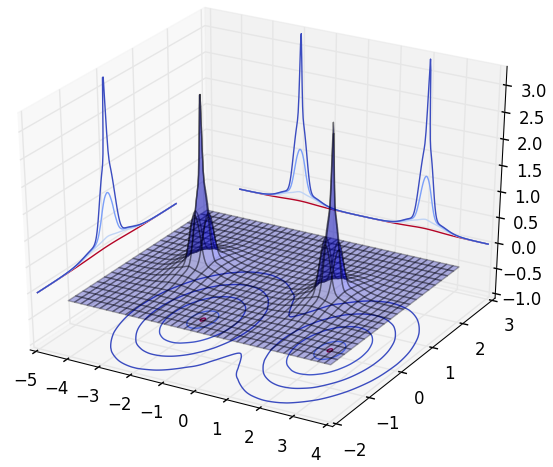
\includegraphics[width=4in]{electron-density-argon-dimer.png}
    \caption{
      Electron density of an argon dimer in the $xy$ plane produced by FHI-aims
      via interface to Python.
    }\label{fig:density-ar2}
\end{figure}

At the time of writing, two example hooks are provided in
\verb+aimsfiles/utilities/python_hooks/+.
The first one plots the electron density in the $xy$ plane.
Below is a shortened glimpse to get a general idea, see the original file for
the complete implementation.
\begin{verbatim}
# ~~ imports ~~

bohr = 0.52917721067

def run(ctx):
    points, rho = ctx.gather_all_grids(['rho'])
    if ctx.rank == 0:  # the grids are gathered only on the root process
        points = points.T  # (3, npts) -> (npts, 3)
        rho = rho.sum(0)  # sum over spin
        in_plane = abs(points[:, 2]) < 1e-10  # points in xy plane
        points = bohr*points[in_plane, 0:2]  # filter & take x, y & scale
        rho = np.log10(1+rho[in_plane])  # filter & log scale
        X, Y = np.mgrid[-4:4:400j, -2:2:200j]  # get rectangular grid
        # interpolate density to rectangular grid
        rho = griddata(points, rho, (X, Y), method='cubic')
        # ~~ matplotlib plotting ~~
\end{verbatim}
Saving this file into \verb+plot-density.py+ and putting
\verb+python_hook plot-density.py parallel+ into \verb+control.in+ produces
Figure~\ref{fig:density-ar2} for an argon dimer.

The other example hook loads Hirshfeld volumes from the output of a previous
FHI-aims calculation.
The parsing part of the hook is executed when FHI-aims parses \verb+control.in+ and
searches for the Hirshfeld analysis section in \verb+hirshfeld.out+.
The actual modification in all processes happens after the normal Hirshfeld
analysis is performed by specifying \verb+python_hook load-hirshfeld.py parallel+.
\begin{verbatim}
import numpy as np

volumes = None

def parse():
    global volumes  # otherwise volumes would be local to function
    with open('hirshfeld.out') as f:
        while 'Performing Hirshfeld analysis' not in next(f):
            pass  # find the Hirshfeld section
        volumes = np.array(list(get_volumes(f)))

def get_volumes(f):
    for line in f:
        if not line.strip():
            return
        if 'Free atom volume' in line:
            free = float(line.split()[-1])
        elif 'Hirshfeld volume' in line:
            hirsh = float(line.split()[-1])
            yield hirsh/free

def run(ctx):
    ctx.hirshfeld_volume[:] = volumes  # replace values in-place
\end{verbatim}
The two-step operation saves computation time if the parsing ended with an
error, since it would abort FHI-aims right after start.
By specifying also
\begin{verbatim}
sc_iter_limit             0
postprocess_anyway        .true.
\end{verbatim}
in \verb+control.in+, one can skip the SCF cycle completely and evaluate
only the van der Waals part of the energy.

\subsection*{Extending the interface}

To extend the range of objects provided by the context object, several simple
steps need to be followed.

\begin{description}

\item[\texttt{python\_interface.f90}] The Fortran type \verb+AimsContext_t+
needs to be extended and the added component needs to be initialized in
\verb+get_aims_context()+ and potentially deallocated in
\verb+destroy_aims_context()+ if it required any allocation.
The latter is of concern only for mapping Fortran types, not simple arrays.
\item[\texttt{cffi/python\_interface.h}] The corresponding C struct
\verb+AimsContext_t+ needs to be updated accordingly.
When these two steps are done, the object is already available in its raw form
in \verb+ctx._c_ctx+.
\item[\texttt{cffi/python\_interface.py}] The initialization of the Python
object \verb+AimsContext+ in \verb+call_python_cffi_inner()+ needs to be
updated accordingly.
For simple arrays, this amounts to simply wrapping the raw C pointers with
Numpy arrays.
For wrapping Fortran types, see how \verb+BatchOfPoints+ and \verb+GridPoints+
are wrapped.

\end{description}

To add new hook labels, add the following lines to the desired location:
\begin{verbatim}
use python_interface, only: run_python_hook, python_hooks

% ...

if (python_hooks%<hookname>%registered) then
    call run_python_hook(python_hooks%<hookname>)
end if
\end{verbatim}
and extend \verb+HookRegister_t+ and \verb+register_python_hook()+ in
\verb+python_interface.f90+ by adding \verb+<hookname>+.
